\section{Own ideas}\label{sec:own_ideas}
\newcommand{\fisher}{Fisher's linear discriminant}

% clustering algos
The majority of clustering-based techniques use algorithms such as $k$-means to generate clusters.
$k$-means' implicit assumptions include that clusters are spherical, isotropic and have roughly the same numbers of samples. % = fester Radius
To loosen these assumptions, other clustering algorithms could be used.
For instance, \ac{dbscan} could be a promising alternative depending on the underlying data.
According to \citet{local_aggr_2019}, \ac{dbscan} scales well to large datasets.
Moreover, it is not necessary to specify the number of clusters $k$ beforehand and 
it is able to detect clusters of arbitrary shapes.
However, \citeauthor{local_aggr_2019} claim that \ac{dbscan} performs poorly on 
high-dimensional data or highly variable density functions.

A combination of different clustering algorithms for methods such as 
\ac{la} \citet{local_aggr_2019} or \ac{pcl} \citet{PCL_2021} could be beneficial.
Since \ac{la} uses $m$ different $k_m$ values for $k$-means clusterings 
to generate hierarchical clusters of different granularity, 
this diversity could be increased by using different clustering algorithms to introduce different cluster shapes.

% AE instead of CNN
Since most techniques discussed in this work have image input data \acp{cnn} seem to be a natural choice for generating embeddings.
However, using \acp{ae} to generate embeddings could be a promising alternative.
Since \acp{ae} are trained using the reconstruction error of the input and output, no additional data is necessary.
This idea is purely speculative and has not been tested yet.

% shortest path in graph
If the data is clustered as displayed in \autoref{fig:graph_svm}a,
the sample pairs within a cluster that have the longest shortest path could be considered as hard positive samples.
Conversely, sample pairs in different clusters with the shortest shortest path could be considered as hard negative samples.

% SNA measures
Even if the input data is not initially a graph, one could transform it into a graph via, for instance, 
the Euclidean nearest neighbour graph discussed in \autoref{subsec:mining_manifolds}.
In computer science, \ac{sna} is a well-known field.
\ac{sna} scientists have developed many measures to analyze graphs.
Therefore, another idea is to use the concept of cliques.
A clique is a subset of vertices of an undirected graph such that every two distinct vertices in the clique are adjacent.
Vertices in a clique are easy positives and reachable vertices outside the clique are hard positives.
This idea would consider the clique vertices to be interchangeable.

% SVM: SV as negative samples
Another idea is to use \acp{svm} to generate hard samples as visualized in \autoref{fig:graph_svm}b.
Initially, the data is split into two classes. 
Since true class labels are not available in \ac{cl}, clustering results are used as a proxy.
Then, a \ac{svm} is trained on the data.
After training, the decision boundary is determined such that the margin is maximal.
The samples that are closest to the decision boundary are considered as \acp{sv}.
Each pair of \acp{sv} from different sides of the decision boundary is considered a (hard) negative pair.
Similarly, distant samples from the decision boundary and their \acp{sv} are considered hard positive pairs.
Since \ac{svm} is a binary classifier, $k>2$ clusters would have to be handled via
multiple one-vs-the-rest or one-vs-one approaches.

\begin{figure}[h]%
    \centering
    \subfloat[\centering Longest shortest path pairs within a cluster are considered hard positive pairs (green) 
    while shortest path pairs of different clusters are considered hard negative (red).]
    {{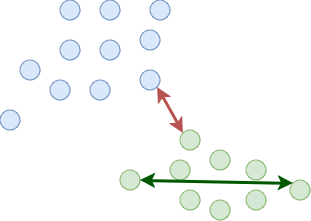
\includegraphics[width=5cm]{images/Cluster_samples.drawio.png} }}%
    \qquad
    \subfloat[\centering Visualization of the \ac{svm} approach. 
    \acp{sv} are displayed as bold points.
    Red arrows denote hard negative pairs while green arrows denote hard positive pairs.]
    {{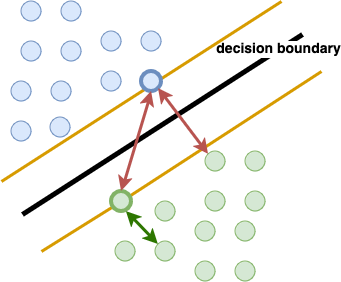
\includegraphics[width=5cm]{images/SVM_samples.png} }}%
    \caption{Samples are displayed as points and their colour denotes their cluster membership.}%
    \label{fig:graph_svm}%
\end{figure}

% Fisher's linear discriminant: overlapping samples
It might be possible to use \fisher{} to generate hard negative samples.
\fisher{} is a linear projection that maximizes the distance between the means of the classes.
Again, two classes are determined via clustering.
As visualized in \autoref{fig:fisher_pca}a, the projected samples of different classes that 
are closest to each other are considered negative samples.

% different PCA axes as negative samples
Since \ac{pca} is a linear transformation, that maximizes the variance of projected data, 
it is the best linear dimension reduction technique in terms of minimization of information loss.
Again, multiple classes are determined via clustering.
The first $n$ \ac{pca} axes are determined for each cluster.
% axes points as samples
Since these axes explain the most variance, equidistant samples lying on these axes could be used as generated samples.
Pairs of projections and their generated axes samples are considered positive samples while 
pairs of projections and samples from different axes are considered negative samples.
This idea is visualized in \autoref{fig:fisher_pca}b.
% cosine similarity
An alternative approach could be to use cosine similarity between vectors spanning \ac{pca} axes of different clusters 
rather than the dot product of two samples, 
because the magnitude of the axes is not of interest but only their direction.

\begin{figure}[h]%
    \centering
    \subfloat[\centering Visualization of the \fisher{} approach.
    To facilitate visualization, the projection of the samples is only implied by dotted lines but not displayed.
    Overlapping projected samples (bold circles) of different clusters are considered hard negative pairs.]
    {{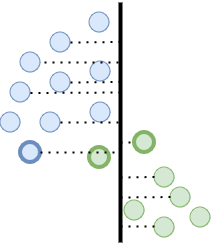
\includegraphics[width=5cm]{images/Fishers_linear_discriminat_samples.png} }}%
    \qquad
    \subfloat[\centering Display of the \ac{pca} idea.
    The first two \ac{pca} axes of each cluster are displayed as lines.
    Green arrows denote positive pairs while red arrows denote negative pairs.]
    {{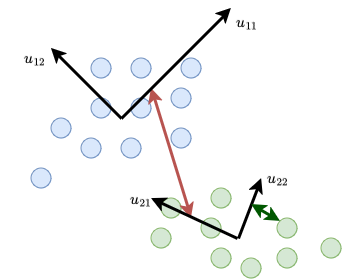
\includegraphics[width=5cm]{images/PCA_samples.png} }}%
    \caption{Samples are displayed as points and their colour denotes their cluster membership.}%
    \label{fig:fisher_pca}%
\end{figure}

% curriculum learning: different sample generation techniques
Moreover, the concept of curricular weighting proposed in \autoref{subsec:curricular_weighting} could be extended.
The notion of hard negative samples being samples in the batch which are more similar to the anchor than positive samples 
proposed in \citet{curricular_weighting_2024} is only one version to generate hard negative samples.
Using other sample generation techniques discussed in this work in combination with 
the idea of gradually increasing the level of hardness during training could be beneficial.

% drawbacks of ideas: initial clustering
The main drawback of the ideas presented in this section is the initial clustering.
If this clustering produces poor results, i.e. the cluster's samples have different inherent labels, 
all proposed ideas will produce \acp{fn} and thus, the training process will be negatively affected.